\documentclass{bioinfo}
\copyrightyear{2005}
\pubyear{2005}



%=================== package declaration ===================
\usepackage{algorithm}

% for the CLRS style pseudocode typing
\usepackage{clrscode3e}





\begin{document}
\firstpage{1}

\title[IBD statistics used in demographic inference]{A Simulation-based Approach for Demographic Inference via Identity-by-Descent Haplotype Sharing}
\author[Yang and Hu]{Shuo Yang\,$^{1}$\footnote{to whom correspondence should be addressed} $\ $and Jing Hu\,$^{1}$}
%\author[Yang and Hu\textit{et~al}]{Shuo Yang\,$^{1}$\footnote{to whom correspondence should be addressed} $\ $and Jing Hu\,$^{1}$}
\address{$^{1}$Department of Computer Science, Columbia University, New York, NY 10027, USA}

\history{Received on XXXXX; revised on XXXXX; accepted on XXXXX}

\editor{Associate Editor: XXXXXXX}

\maketitle

\begin{abstract}

\section{Motivation:}
With the fast development of genome sequencing technology, there is increasing amount of genomic data ready for analysis. How to interpret these data then becomes a challenge for genetic researchers. When the population evolutionary model becomes more and more realistic but complicated, theories that can precisely explain the data are very hard to develop or to apply even with much mathematical approximation. As a result, computer simulation gives us a new and more powerful direction for genetic analysis, in the context of explaining the evolutionary model of the samples, or demographic inference.

\section{Results:}
In this project, we evaluated a new statistic within the simulation-based framework for demographic inference via Identity-by-Descent (IBD) haplotype sharing. The new statistic characterizes the average sharing of IBD among samples, and is natural to be used in haplotype imputation. We also combined the new statistic with the well-studied IBD length (number) distribution statistic, to demonstrate that simple combining won't improve the precision of the inference. Our approach that utilizes the IBD statistics for demographic inference will work better for recent history inference compared to the traditional site frequency spectrum (SFS) based methods, as long haplotype sharing contains more information about recent population history via chromosome recombination other than mutation. Additionally, our project will become a model that statistics of genetic data can be used in simulation analysis in order to uncover interesting and important genetic meanings.


\section{Availability:}
All source code is freely available for download at https://github.com/morrisyoung/CompGenome.



\section{Contact:} \href{sy2515@columbia.edu}{sy2515@columbia.edu}
\end{abstract}






\section{Introduction}

Nowadays, population genetics has entered a new era, in which the need for simulation-based methods is strengthened again and again. Complicated genetic phenomenon can sometimes be described by brief and gentle mathematics. However, this sometimes can be very hard to realize, especially when the demographic model of observed genetic data is too complicated to simplify via mathematical approximation. In that case, we can?t always use analytic approach to tackle the problem of explaining genetic data, so a simpler but still effective method will then be greatly favored. Researchers in this field then proposed the simulation-based method, like the one in~\cite{Excoffier2013}, which is actually an important component in other related research.

However, there are two main challenges in such an approach. The first one is to choose the appropriate statistics to apply into the simulation framework, which will, to some extent, determine the effectiveness of the simulation-based approach. And the second one is to find an efficient way to simulate and infer, which will possibly limit the broad applicability of one proposed method.

As we have seen in~\cite{Excoffier2013}, site frequency spectrum (SFS) has already been fluently used in such works. They applied the SFS into demographic inference to explain the observed genomic data, which was demonstrated both accurate and efficient especially for very complicated models. Also, the composite likelihood method they used is a very flexible one in such works, which may be further exploited in other works. However, the SFS based method will dramatically lose its power when we are specifically interested in the recent history of the genetic data, during which time there is long haplotype sharing, and the SFS is not as statistically meaningful under such short history as it is from long evolution history. Enlightened by that, we plan to use those long haplotype sharing between two reportedly unrelated individuals among a cohort, formally defined as Identity-by-Descent (IBD), with its rich statistics into the simulation framework, for explaining the recent history of the genomic data.

Benefiting from some well-built theories used to describe the evolution models in population genetics, such as sequential Markov coalescent (SMC) and SMC' (see~\cite{McVean2005} and~\cite{Marjoram2006}), we can rapidly simulate the genetic data according to various population models with high confidence in their accuracy. Lots of downstream statistics can then be extracted via computational approaches. Our work, at this stage, is to integrate our simulation and statistical inference works into such existing simulators, to evaluate the effectiveness of some statistics used in such demographic inference, and to ultimately build a framework with appropriate computational power needed, dedicated for simulation-based demographic inference of recent population history.




\section{Approach}

We will start from very simple population models -- constant population size model, and the bottleneck population model (Figure~\ref{fig:model}). They are simple enough to be a good start for such exploratory research. Also, especially for the second one -- the bottleneck model, it's said to be consistent with what really happened in recent history for some human populations. The parameter we hold interests in the constant population size model is the population size $N$ (or $N_e$ in some traditional literature). In the bottleneck model, we are interested in the following parameters:

\begin{enumerate}
\item $NA$: ancient population size;
\item $NC$: current population size;
\item $TB$: time to bottleneck event;
\item $NB$: bottleneck population size; or $T$: bottleneck duration;
\item $\frac{T}{NB}$: bottleneck strength
\end{enumerate}

For all these parameters, their default values in our testing are: $NA=10000$, $NC=10000$, $TB=30$, $NB=200$, $T=10$.

\begin{figure}[h]
\centerline{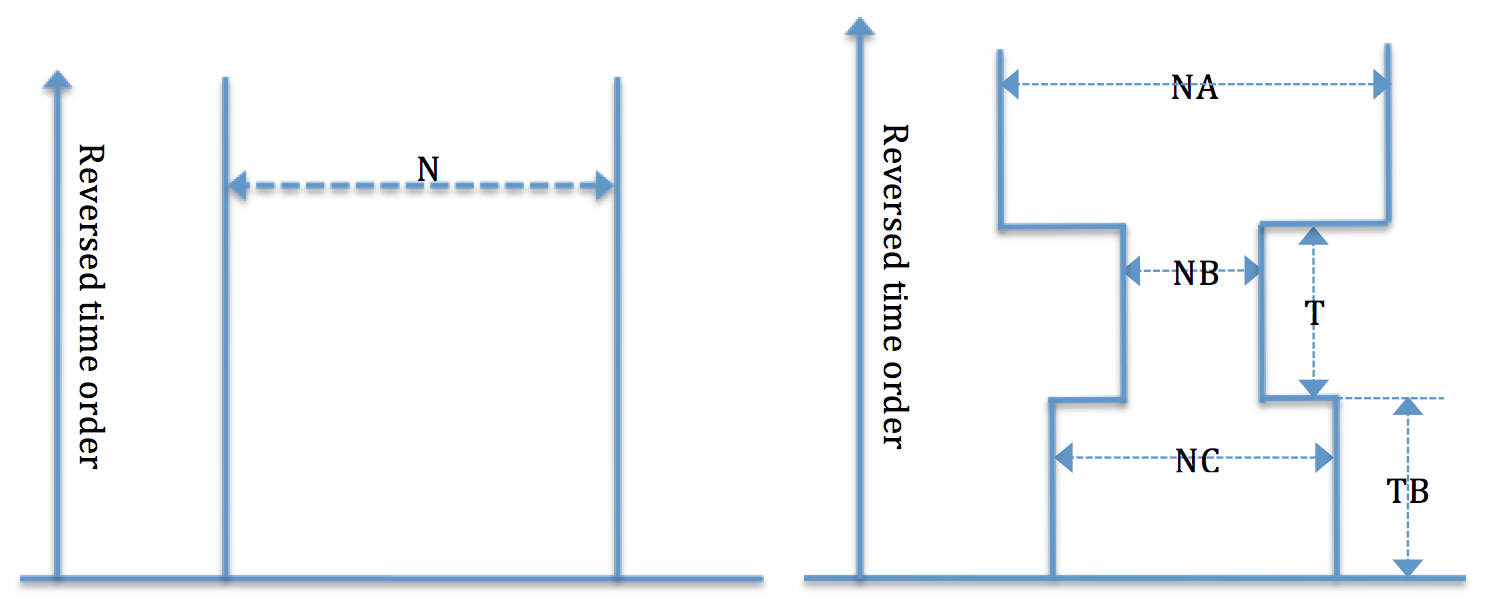
\includegraphics[width=240pt, height=100pt]{model}}
\caption{Two models to be evaluated. The left one is the simple constant population size model, which is not very realistic in practice. The right one is the bottleneck model, which is consistent with true human population history for some populations (and the big trend).}\label{fig:model}
\end{figure}

In all of these models, as old works are based on IBD segment number distribution (results not shown), we will here use a new statistic -- average IBD sharing statistic, in the inference framework, and try to compare this with the old results from old statistic. See~\ref{fig:newstats}~\cite{Carmi2014} for the explanation of this statistic. The origin of this statistic is genome sequencing. Intuitively, the more sequenced individuals from a population we have in hands, the larger proportion of cohort-sharing IBD segments will present, meaning that the average fraction of the genome that can be imputed via the sequenced chromosomes increases. Though it's a natural statistic for genome sequencing, this statistic gives us a full and better description of the cohort-sharing properties of IBD segments, and how it is shaped by historical events, which can therefore be exploited by demographic analysis of population genetics.

\begin{figure}[h]
\centerline{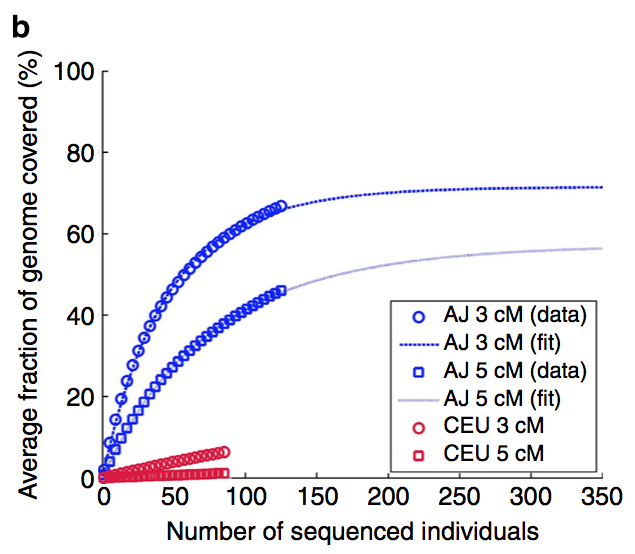
\includegraphics[width=160pt, height=140pt]{NewStats}}
\caption{The average sharing of IBD with increased number of reference genomes within a cohort.}\label{fig:newstats}
\end{figure}

To get these statistics, we will use simulations, as we don't have theories for the statistics (especially for the new one) under these models. That's also why we call our method as simulation-based method.




\begin{methods}
\section{Methods}

We will use \textit{fastsimcoal2}~\cite{Excoffier2013} to simulate the genomes according to different population parameters. We will also use \textit{IBDdetection}~\cite{Yang2015} to extract the ground-truth IBD segments from simulated Ancestry Recombination Graph (ARG). The IBD segments used in the demographic analysis should be ground-truth, as they will act as the reference genomes, and that's why we directly extract IBD segments from ARG other than the sequence data. These software are enough for evaluation purpose, and we actually didn't practically infer the parameters (that's less meaningful than the evaluation first of all).

We will use the procedure in Algorithm~\ref{algo:newstats} to generate the new statistic with simulations. Specially, $\Theta$ is the population parameters we use to generate the samples and the IBD statistics. It should contain the value of $N$, $NA$, $NC$, $NB$, $T$ and $TB$. $n$ is the sample size in the simulation. The output of the procedure is the new statistic: average fraction of IBD cohort-sharing corresponding to the case of $x$ reference genomes are sequenced, where $x$ is equal to $[5,10,...,n]$.

\begin{algorithm}
\caption{IBD average sharing statistic generating}
\label{algo:newstats}
\vspace{-0.32cm}  % this vspace should be legal, because it's inside another module (algorithm box)
\begin{codebox}
\Procname{$\proc{NewStats}(\Theta, n)$}
\li	$Stats=\{5:0, 10:0, 15:0, ... , n:0\}$
\li	$Simu=20$\Comment{$20$ simulations are used to average}
\li	$Iter=50$\Comment{$50$ samplings are used to average}
\li \For $i=1,2,...,Simu$
\li	\Do	\textit{fastsimcoal2}($\Theta$)
\li		\For $j=1,2,...,Iter$
\li		\Do \For $k=5,10,15,...,n$\Comment{where statistics are picked}
\li			\Do randomly sample $1$ genome, as $g$
\li				randomly sample $k$ genomes, as $G$
\li				$IBDdetection$($g$), $IBDdetection$($G$)
\li				$f=$ fraction of co-sharing between $g$ and $G$
\li				$Stats[k]+=f$
			\End
		\End
	\End
\li	$Stats=\frac{Stats}{Simu \times Iter}$
\li	return $Stats$
\end{codebox}
\vspace{-0.35cm}  % this vspace should be legal, because it's inside another module (algorithm box)
\end{algorithm}

Specially, to average the statistics we get from simulation, we run $20$ simulations with the specified population parameters. Also, for each $k$ (the number of reference genomes that are sequenced), we randomly sample $50$ times (for both the target genome and these $k$ genomes). With this strategy, we hope to get the statistics as what they actually are.

Also, to get the distance between two statistics, we will utilize Algorithm~\ref{algo:distance} (squared distance). In this study, we will draw the distance curve (or surface if two parameters are estimated jointly), to evaluate whether the minimum distance between guessed parameter value and the true parameter value exactly happens in the true value. If that is the case, we can optimize along the distance curve (or surface) to retrieve the true parameter value, and that's what we call effective demographic inference.

\begin{algorithm}
\caption{distance calculating from IBD cohort-sharing}
\label{algo:distance}
\vspace{-0.32cm}  % this vspace should be legal, because it's inside another module (algorithm box)
\begin{codebox}
\Procname{$\proc{Distance}(Stats_1, Stats_2)$}
\li	$dis = 0$
\li	\For $k=5,10,15,...,n$
\li	\Do	$dis += (Stats_1[k] - Stats_2[k])^2$
	\End
\li	return $dis$
\end{codebox}
\vspace{-0.35cm}  % this vspace should be legal, because it's inside another module (algorithm box)
\end{algorithm}

In the final stage, after comparing the new statistic with the old one, we will try to combine them to see whether it will help. As the new statistic provides us extra and independent information about the population evolution (but not necessarily perfect information), combining it with the old one to make them contribute roughly equally may characterize the population history better. We will discuss later about how to combine them in an empirical but effective way.



\end{methods}

\section{Results}

We will show, with the new average IBD sharing statistic, all the parameters we evaluated with their distance curve (or joint distance surface). Also, we will show the combined distance curve when considering the two statistics at the same time. We worked on the constant size population model, and the bottleneck model.

\subsection{Constant population size model}

Figure~\ref{fig:dis_N} shows us different statistics of average IBD sharing under different population size $N$. The trend of the distributions across different value of $N$ tells us that inference is feasible for this parameter, and we then show the distance curve for different $N$ compared to the true value, say $N = 5000$, in Figure~\ref{fig:like_N}. This parameter is also feasible to estimate with old statistic -- IBD number distribution (data not shown).

\begin{figure}[h]
\centerline{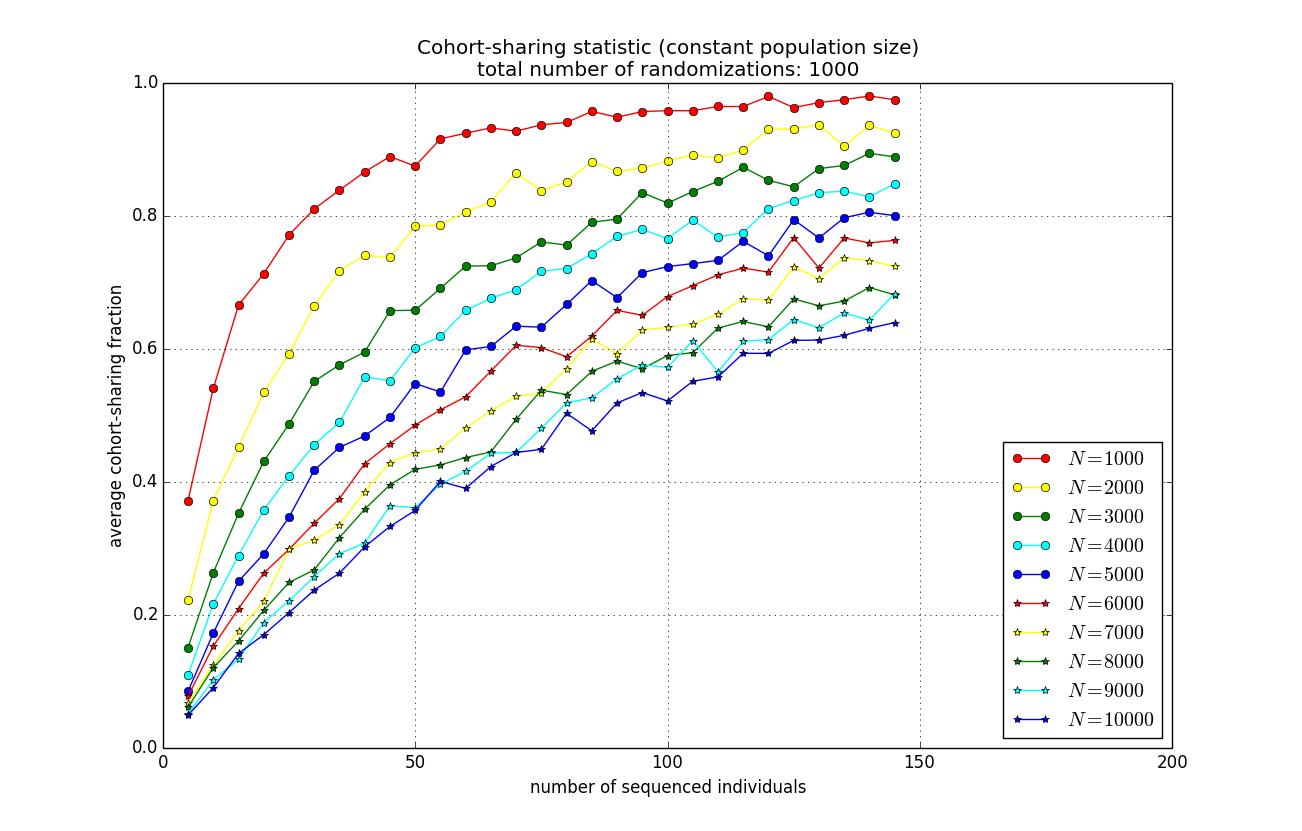
\includegraphics[width=290pt, height=200pt]{dis_N.png}}
\caption{Different statistics of average IBD sharing across different $N$.}\label{fig:dis_N}
\end{figure}

\begin{figure}[h]
\centerline{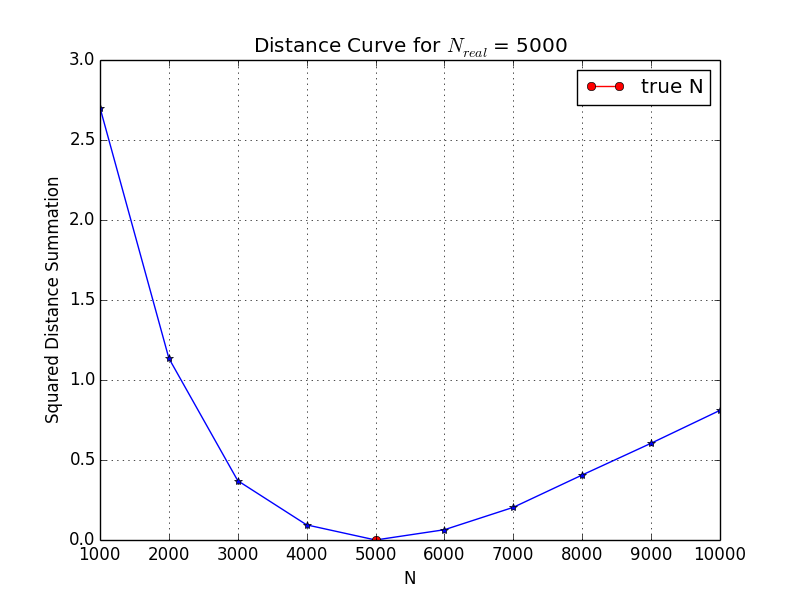
\includegraphics[width=280pt, height=200pt]{like_N.png}}
\caption{The corresponding distance curve for Figure~\ref{fig:dis_N} if true parameter is $N=5000$. In this case, minimum distance happens exactly in the true parameter value.}\label{fig:like_N}
\end{figure}


\subsection{Bottleneck model}

Now we will work on the bottleneck model, in which we are interested in $NA$, $NC$, $NB$, $T$ and $TB$, or some kinds of combinations among them. For evaluating one of these parameters, we will set all other parameters as their ``true" value\footnote{the value used in the model to generate the ``observed" samples.}. If we evaluate two parameters jointly, we will set all other parameters as their ``true" value, and only vary the two jointly.

$NA$ and $NC$ are the two parameters we naturally hold interests in, as population size always (but not all the time as we will see) greatly affect the evolutionary process of the population. In Figure~\ref{fig:dis_NA} and~\ref{fig:dis_NC}, we show their distance curve, which seems not optimistic. This is within out expectation, as in this bottleneck model, the IBD sharing among current genomes seems to be greatly shaped by the bottleneck event itself, other than the ancient/current population size. So we hold more interests to interpret the bottleneck event with the observed IBD sharing. (the same result for the old statistic IBD segment number distribution; data not shown).

\begin{figure}[h]
\centerline{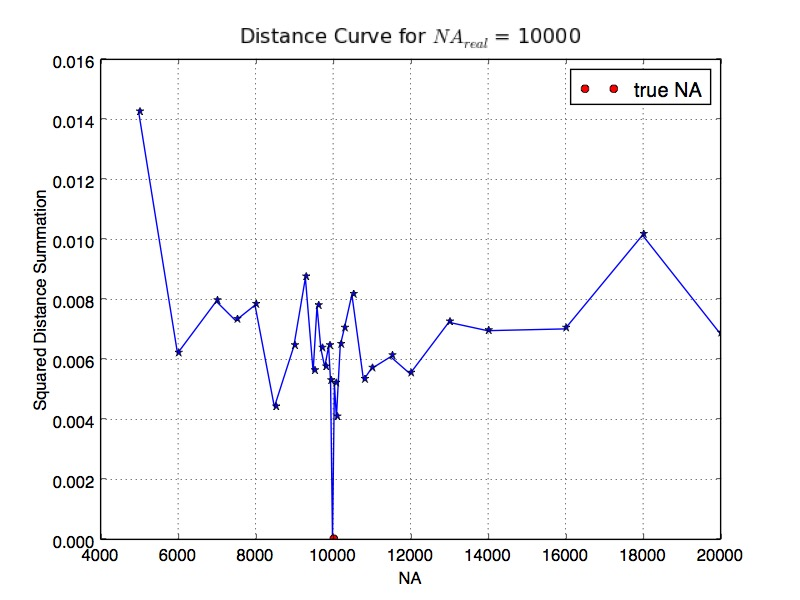
\includegraphics[width=280pt, height=200pt]{like_NA.jpg}}
\caption{The distance curve for $NA$ if true parameter is $NA=10000$. In this case, minimum distance doesn't necessarily happen in the true parameter value, as this curve is not convex. Indeed, it's not even smooth at all.}\label{fig:dis_NA}
\end{figure}

\begin{figure}[h]
\centerline{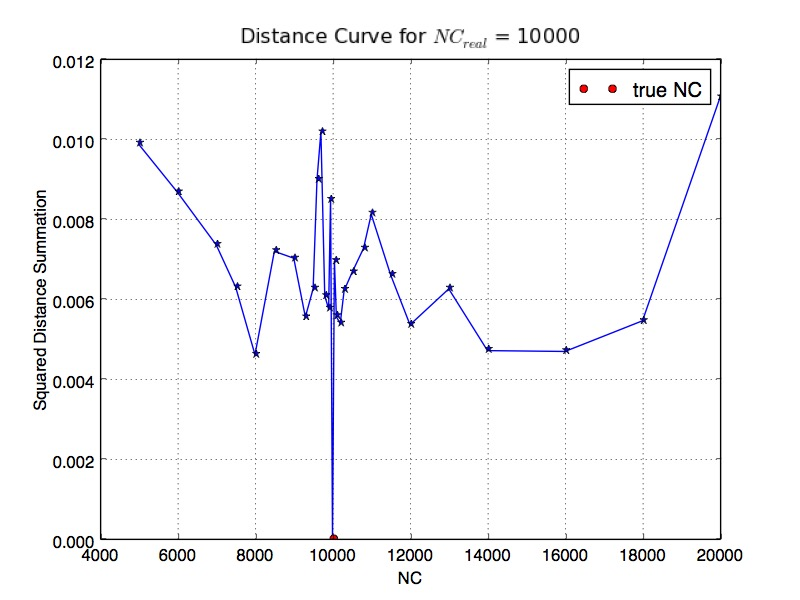
\includegraphics[width=280pt, height=200pt]{like_NC.jpg}}
\caption{The distance curve for $NC$ if true parameter is $NC=10000$. In this case, minimum distance doesn't necessarily happen in the true parameter value, as this curve is not convex. Indeed, it's not even smooth at all. This is similar to the curve of $NA$.}\label{fig:dis_NC}
\end{figure}

As we are now more interested in the bottleneck event itself, we start from $TB$, which is the time point when this bottleneck event happened. See Figure~\ref{fig:dis_TB}. From the figure, we can say this parameter is also unfeasible to estimate. This is not the same case for the IBD segment number distribution statistic, in which $TB$ is feasible to estimate.

\begin{figure}[h]
\centerline{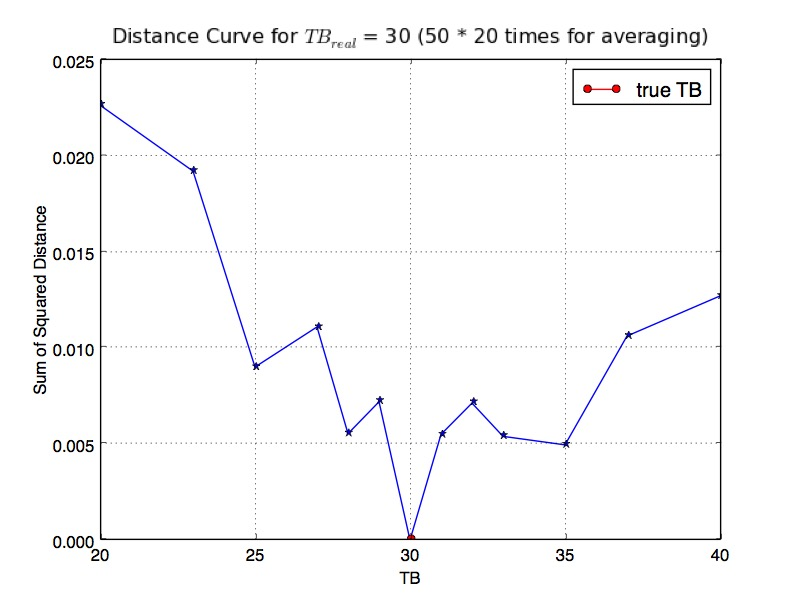
\includegraphics[width=280pt, height=200pt]{like_TB.jpg}}
\caption{The distance curve for $TB$ if true parameter is $TB=30$. In this case, minimum distance doesn't necessarily happen in the true parameter value, as this curve is not convex. Indeed, it's not even smooth at all.}\label{fig:dis_TB}
\end{figure}

However, according to our result of IBD segment number statistic, such imperfect $TB$ won't affect the other two parameters in the bottleneck event -- $NB$ and $T$, so we next show the joint distance curve (surface) for $NB$ with $TB$, and $T$ with $TB$, in Figure~\ref{fig:dis_NBTB} and~\ref{fig:dis_TBT}. The two parameters also show a same trend that, without perfect information of $TB$, we can still estimate them, if we set other parameters (including $NB$ and $T$) as their true value.

\begin{figure}[h]
\centerline{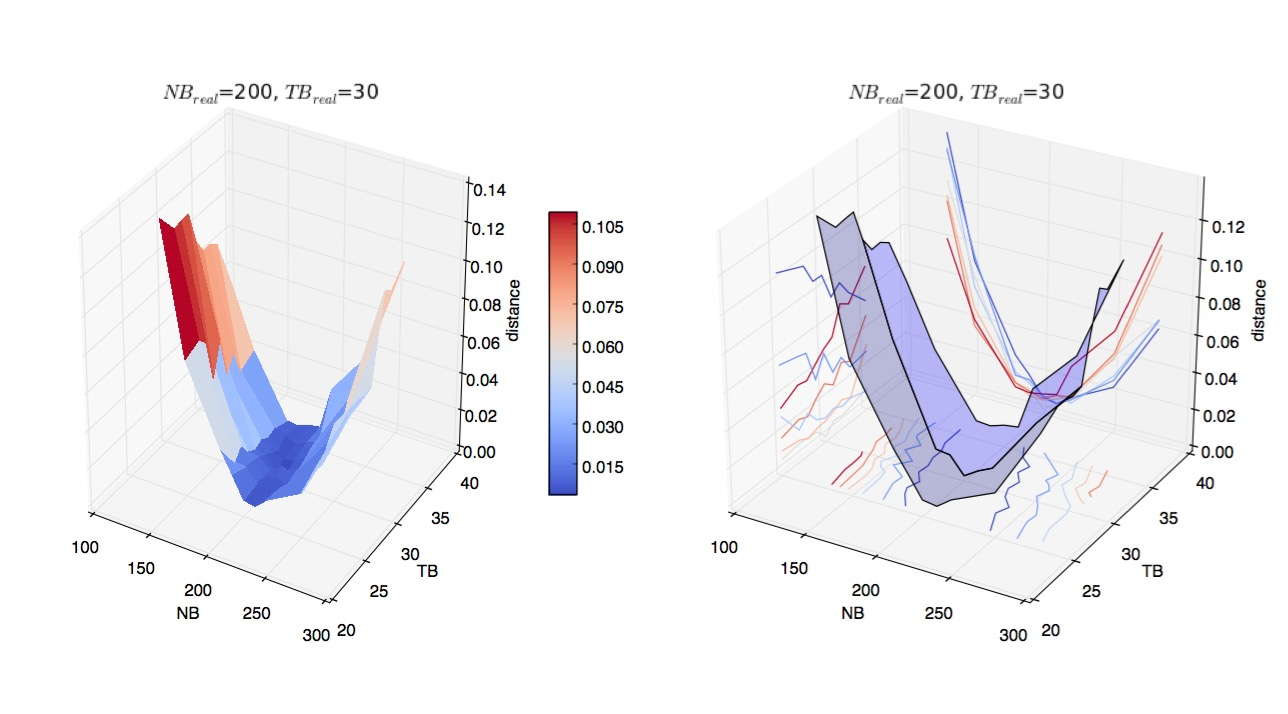
\includegraphics[width=270pt, height=150pt]{like_NBTB.jpg}}
\caption{The joint distance surface for $NB$ and $TB$ if true parameter is $NB=200,TB=30$. We can see from the surface that, $TB$-dimension is always noisy (not estimatable), while $NB$-dimension is always good enough to estimate no matter what $TB$ is.}\label{fig:dis_NBTB}
\end{figure}

\begin{figure}[h]
\centerline{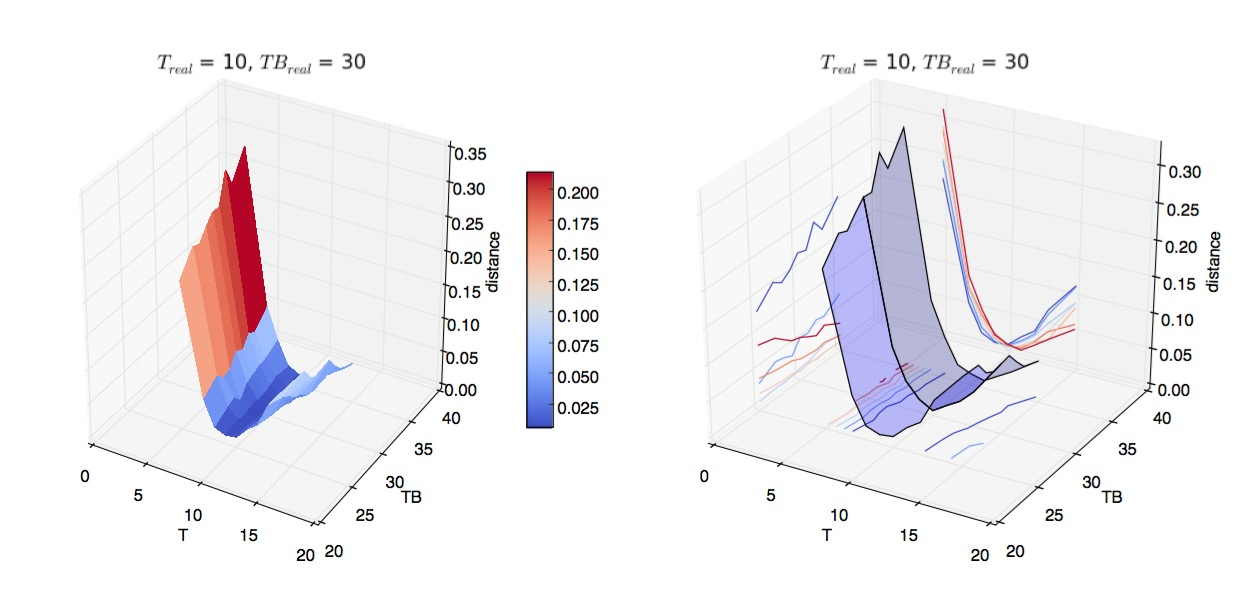
\includegraphics[width=270pt, height=150pt]{like_TBT.jpg}}
\caption{The joint distance surface for $T$ and $TB$ if true parameter is $T=10,TB=30$. We can see from the surface that, $TB$-dimension is always noisy (not estimatable), while $T$-dimension is always good enough to estimate no matter what $TB$ is.}\label{fig:dis_TBT}
\end{figure}

In the above evaluation, whenever we evaluate $NB$ or $T$, we indeed set $T$ or $NB$ (the other parameter) to its true value. Now we will jointly consider this two parameters -- $NB$ and $T$. See Figure~\ref{fig:dis_NBT}. This is, again, similar to what we saw from the IBD segment number distribution. There is a diagonal in the joint parameter space, which seems to achieve the global minimum value all the time. That is to say, under the current model, the separate true value of $NB$ and $T$ are not able to be determined, while their ratio is.

\begin{figure}[h]
\centerline{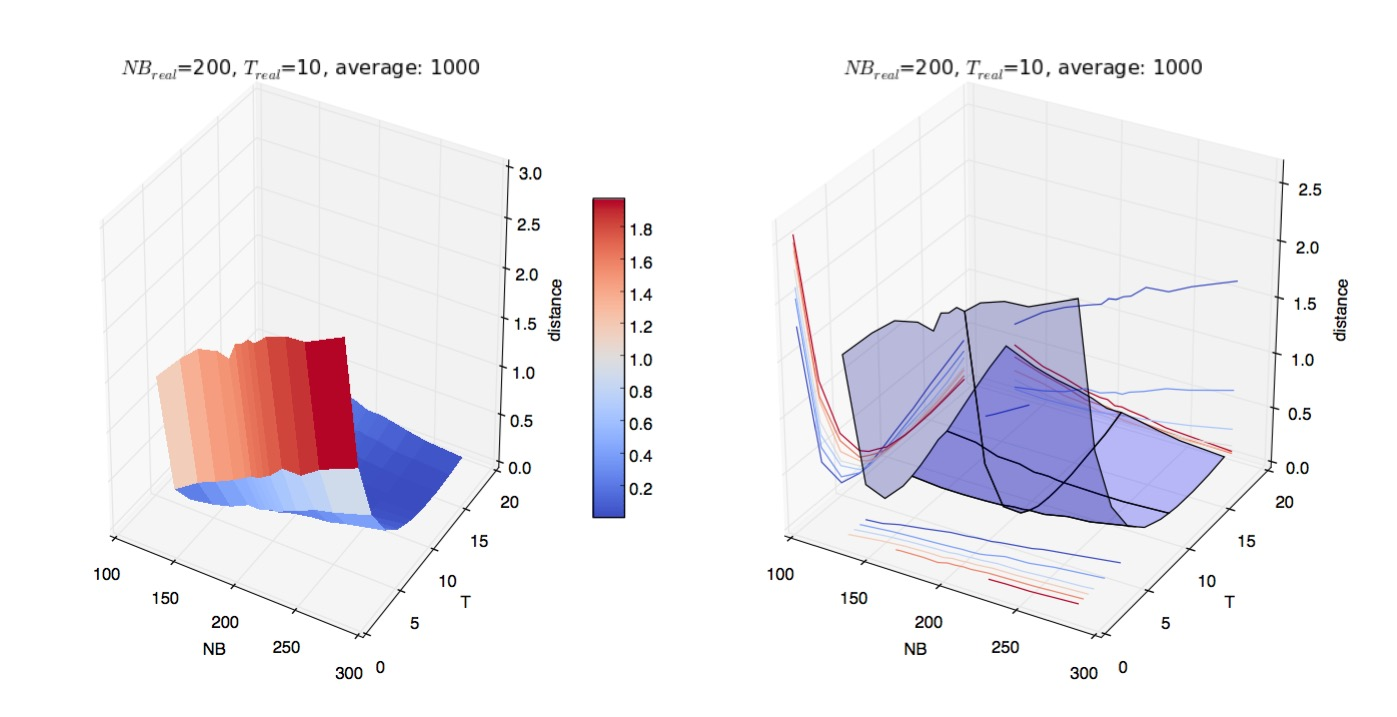
\includegraphics[width=270pt, height=150pt]{like_NBT.jpg}}
\caption{The joint distance surface for $T$ and $TB$ if true parameter is $T=10,TB=30$. It seems that the ratio of this two parameters matters in minimizing the distance.}\label{fig:dis_NBT}
\end{figure}

We now try to evaluate whether or not the ratio of $NB$ and $T$, say $\frac{T}{NB}$ is feasible to estimate. We set $T$ to different values, say, $5$, $10$ and $20$ ($10$ is not shown below), and we try to draw the joint distance surface of $NB$ and $TB$, to see whether the ratio of $\frac{T}{NB}$ can be retrieved with different value of $T$. See Figure~\ref{fig:dis_NBTBT5} and~\ref{fig:dis_NBTBT20} for more details. The results here is not so optimistic, as there are two following points. So the new statistic is still not better until now.

\begin{enumerate}
\item The estimation of $\frac{T}{NB}$ ($NB$ in practical evaluation) seems feasible, but greatly biased by the value of $TB$; such estimation is indeed better than this with the old IBD segment number distribution statistic, which we will discuss later;
\item The joint estimation of $TB$ in this case is not feasible, but it's indeed feasible with the old statistic and we will discuss that later.
\end{enumerate}

\begin{figure}[h]
\centerline{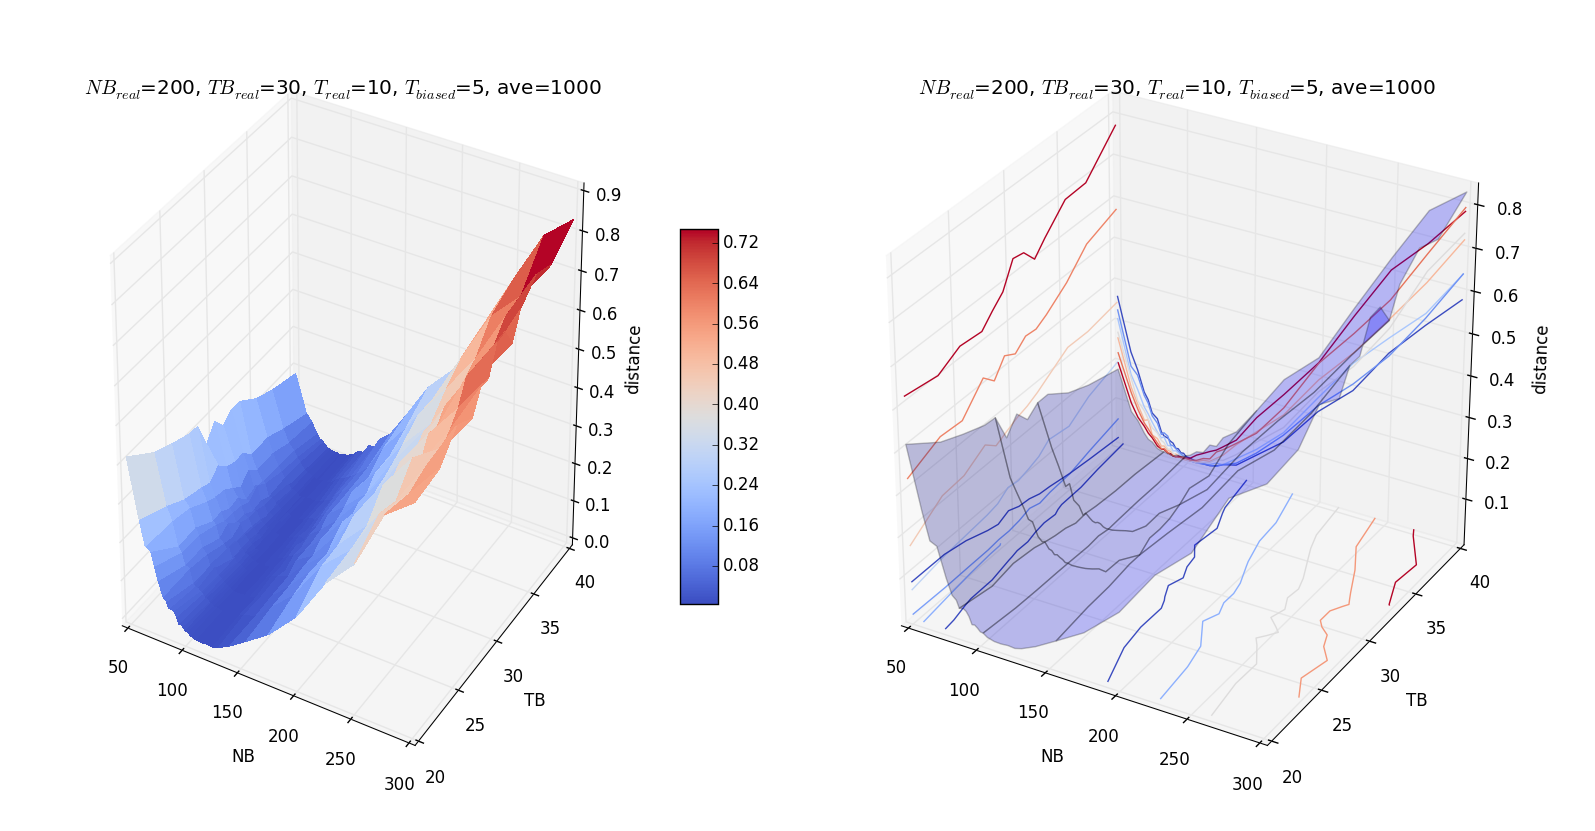
\includegraphics[width=270pt, height=150pt]{like_NBTBT5_2.png}}
\caption{The joint distance surface for $NB$ and $TB$ if true parameter is $NB=100$ (assuming constant $\frac{T}{NB}$, and $T$ is set to $5$), $TB=30$. We can see from the surface that, $TB$-dimension is always noisy (not estimatable), while $NB$-dimension seems good but still biased a lot.}\label{fig:dis_NBTBT5}
\end{figure}

\begin{figure}[h]
\centerline{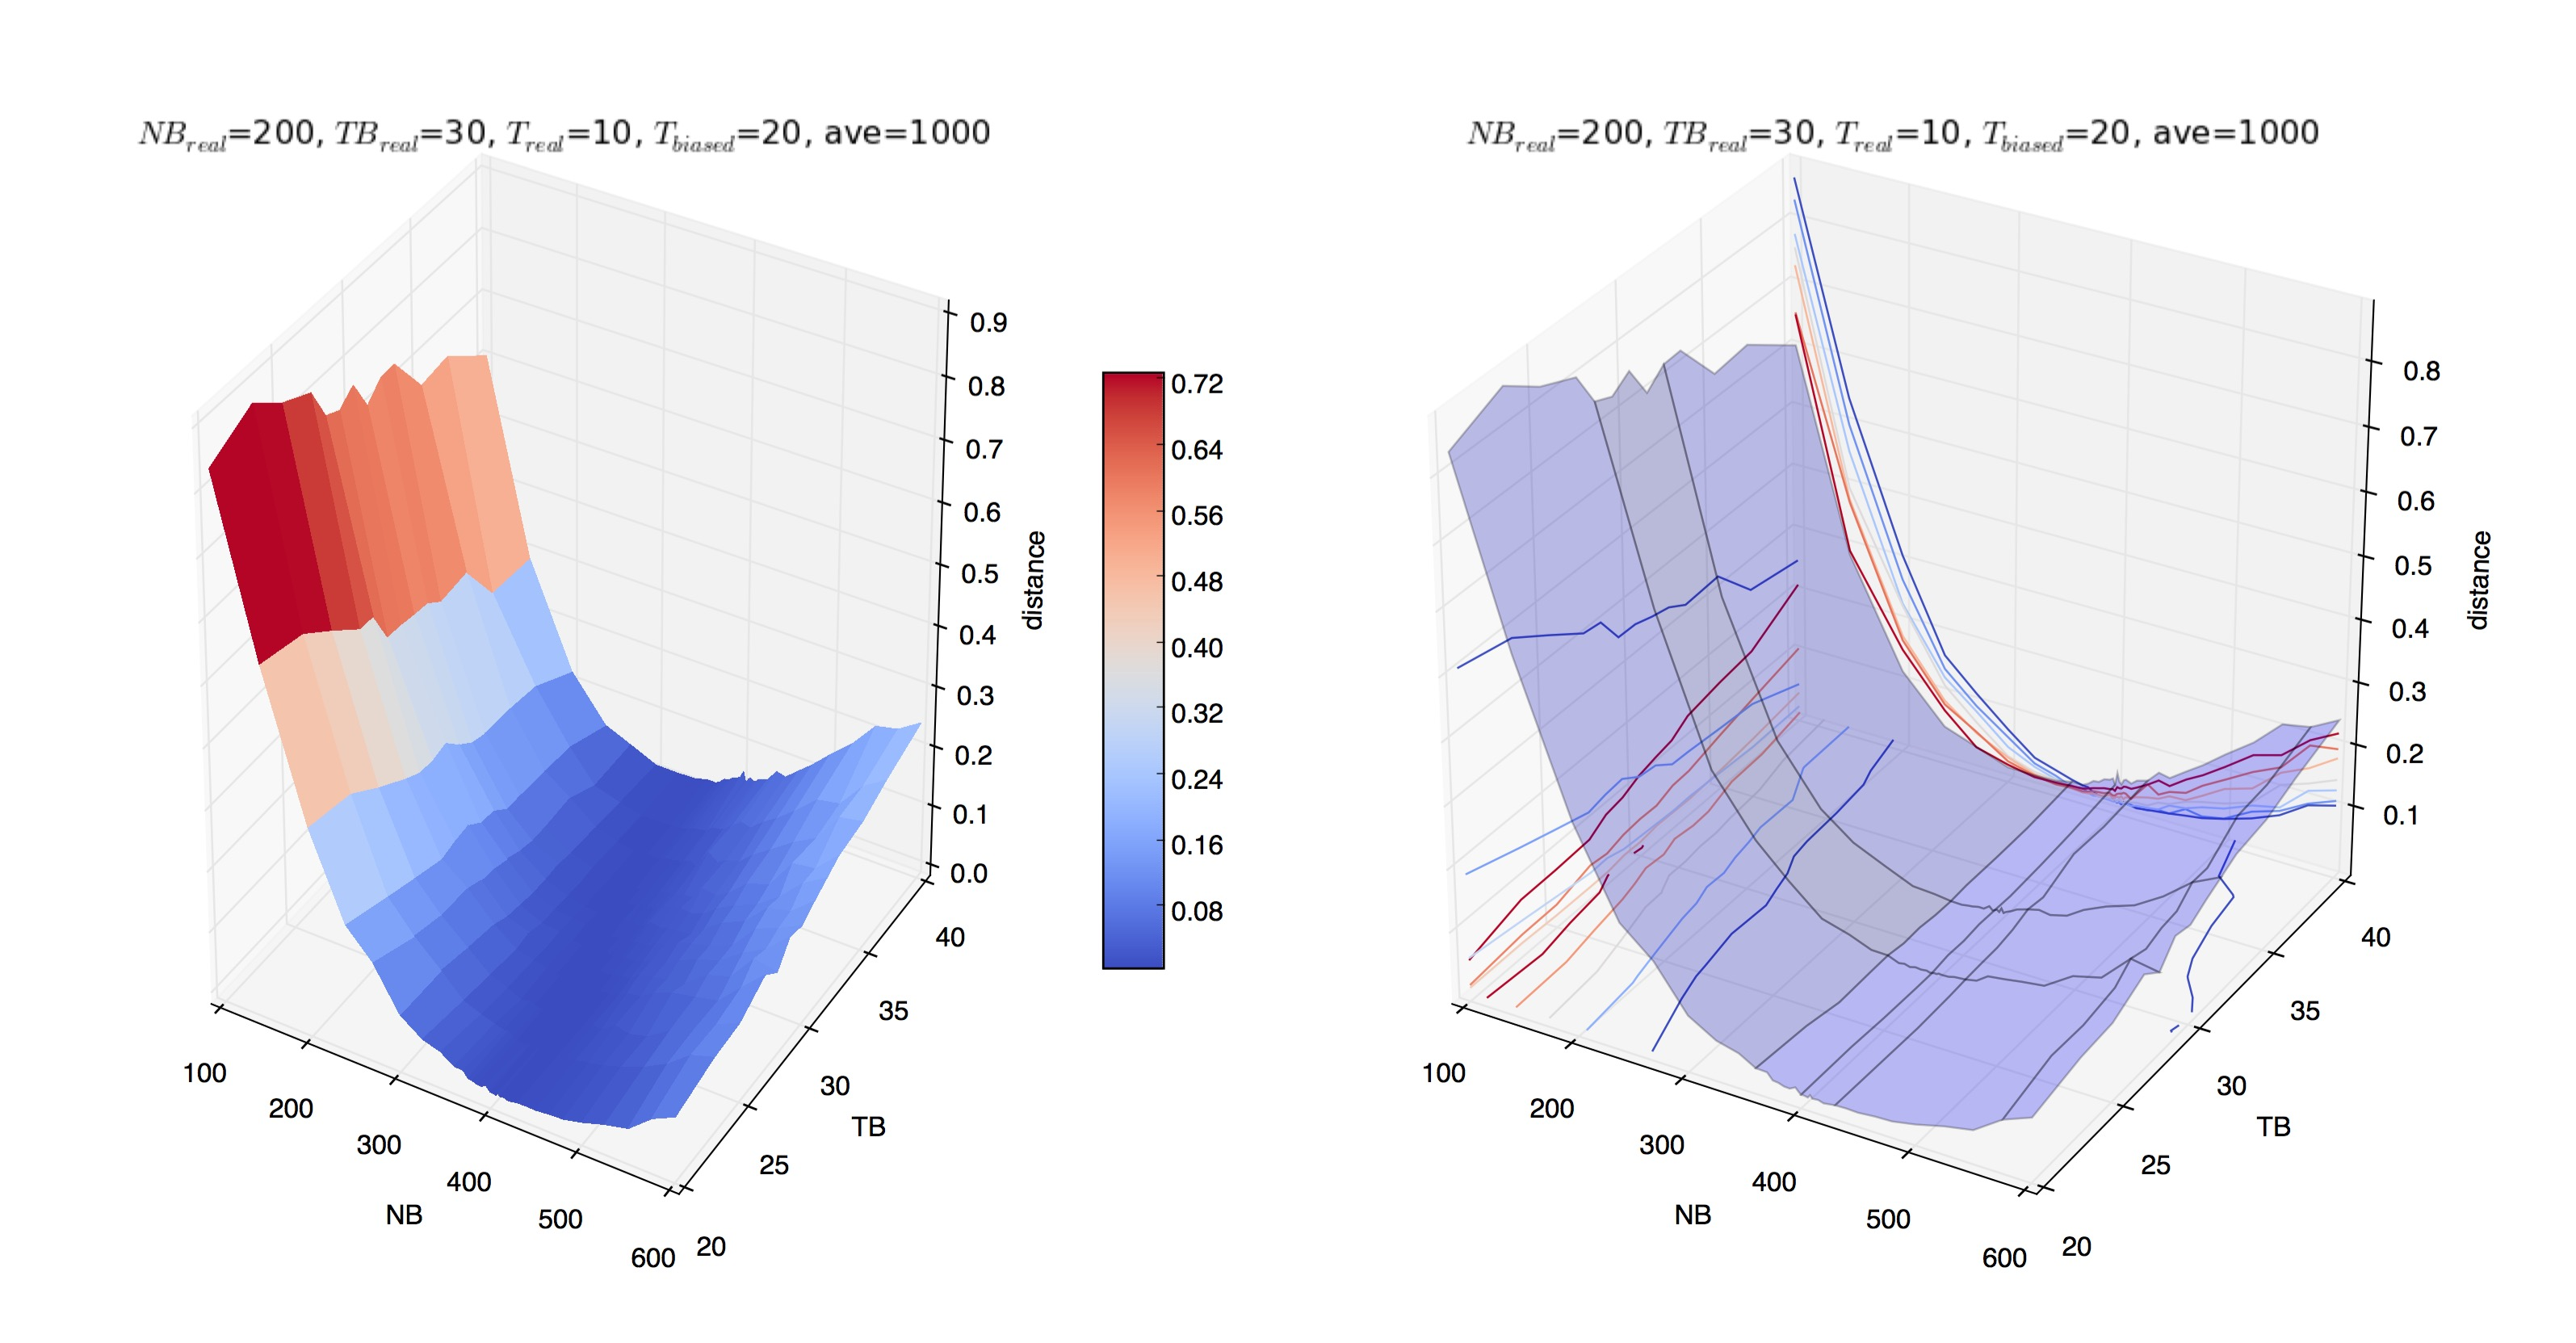
\includegraphics[width=270pt, height=150pt]{like_NBTBT20_2.jpg}}
\caption{The joint distance surface for $NB$ and $TB$ if true parameter is $NB=400$ (assuming constant $\frac{T}{NB}$, and $T$ is set to $20$), $TB=30$. We can see from the surface that, $TB$-dimension is always noisy (not estimatable), while $NB$-dimension seems good but still biased a lot.}\label{fig:dis_NBTBT20}
\end{figure}


\subsection{Combining statistics}

From above discussion, we see that all the parameters here cannot be better estimated with the new statistic -- average IBD sharing statistic. We now try to combine the two statistics to see whether it helps.

The idea about how to combine the two statistics is that, we let them contribute roughly equally to the combined statistic. We can use the \textbf{Max} or \textbf{Mean} of the two statistics to normalize them. Say, for \textbf{Max}, we let \textbf{Max}(stat1) $=x \times$ \textbf{Max}(stat2), where $x=0.4,0.7,1.0,1.3,1.6$. The same for \textbf{Mean}. After doing normalization, we naturally add the distance curves of the two statistics together, to see whether it's smoother, or more convex than before. In practice, this combination doesn't help even a little. And here we only use two simple samples to demonstrate that, $NA$ and $NC$. See Figure~\ref{fig:dis_com_NA} and Figure~\ref{fig:dis_com_NC}.

\begin{figure}[h]
\centerline{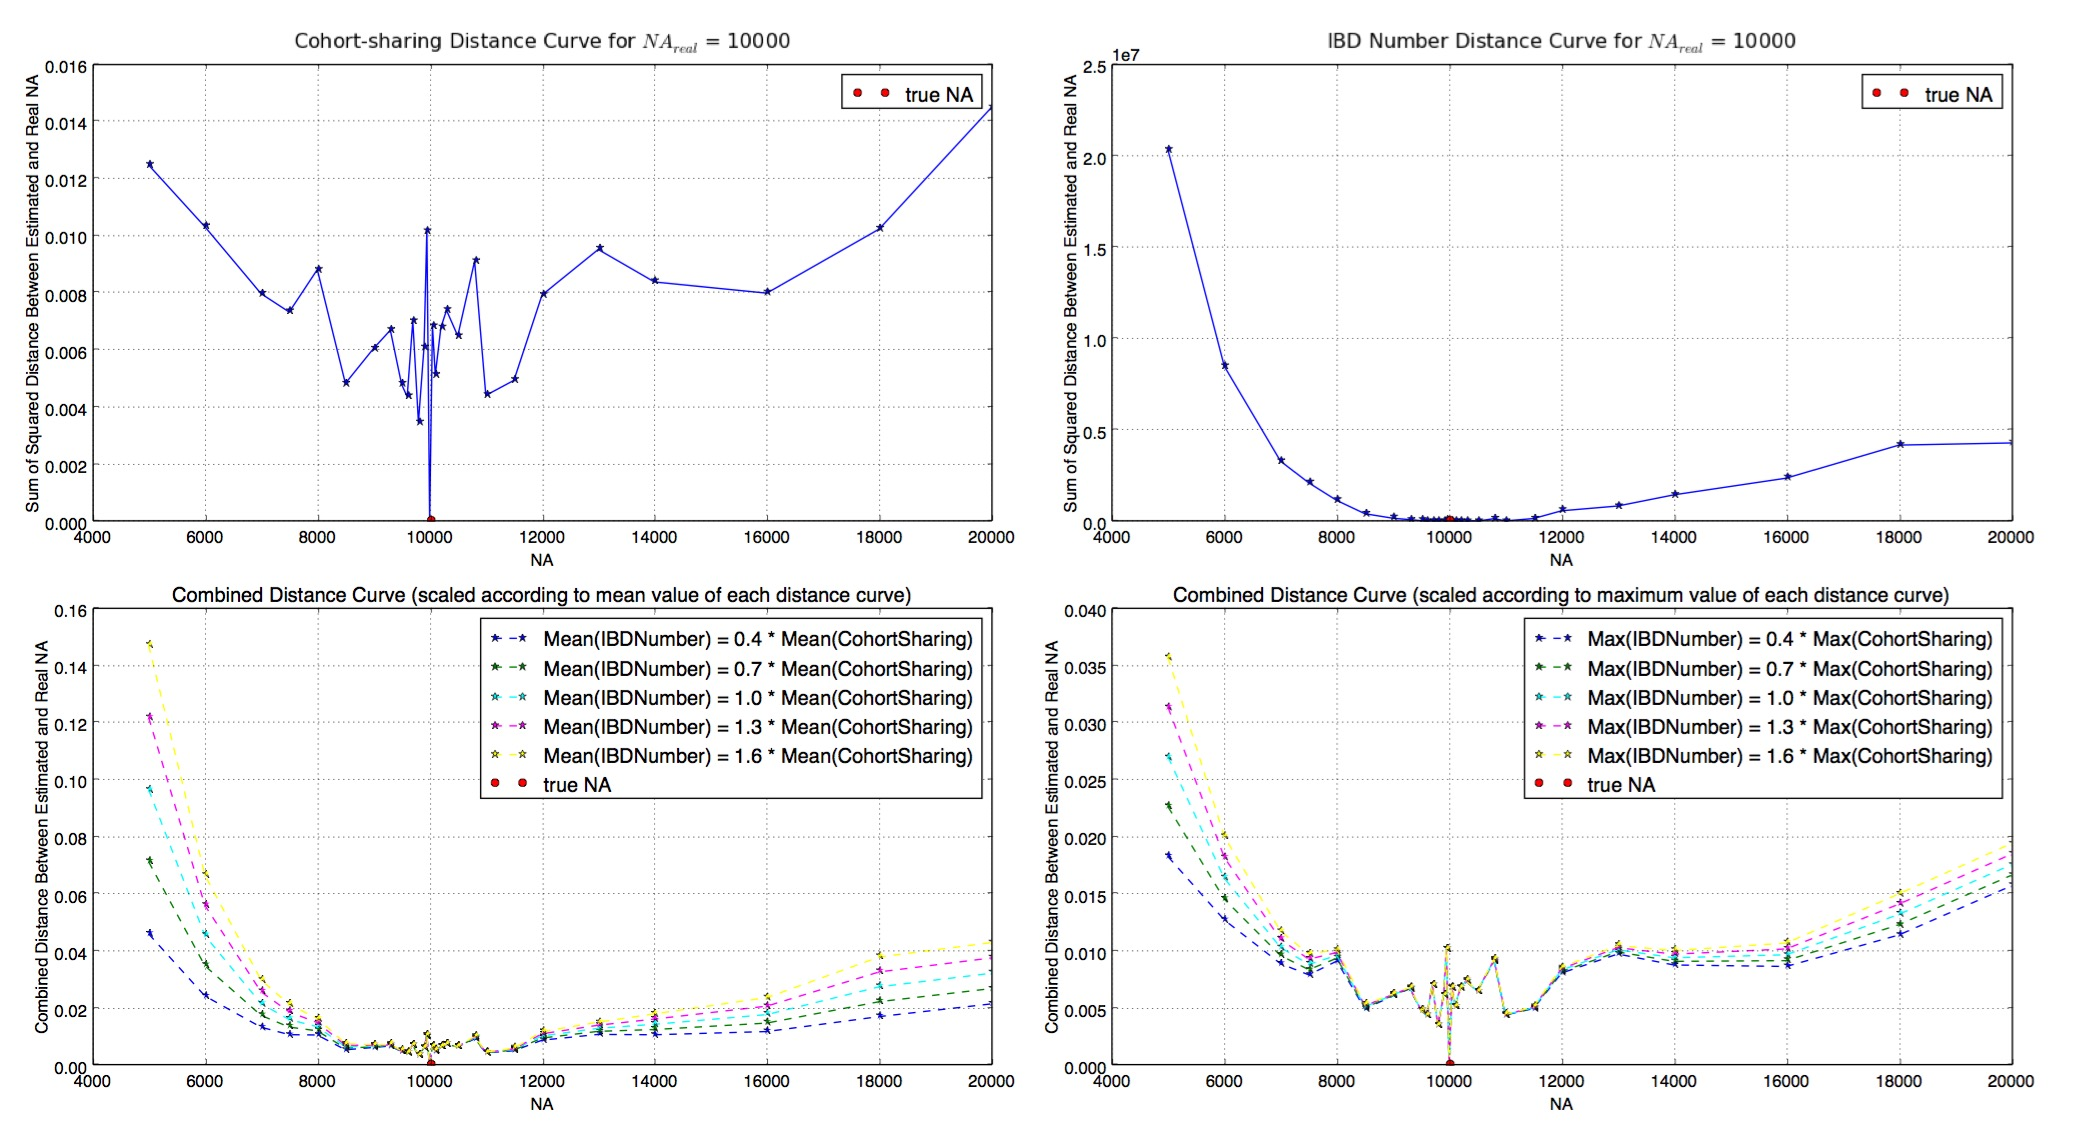
\includegraphics[width=280pt, height=170pt]{like_com_NA.jpg}}
\caption{Distance curves for $NA$. The above two curves are the distance curve for average IBD sharing and IBD segment number distribution, and the below two curves are the combined curve according to \textbf{Mean} and \textbf{Max}, respectively.}\label{fig:dis_com_NA}
\end{figure}

\begin{figure}[h]
\centerline{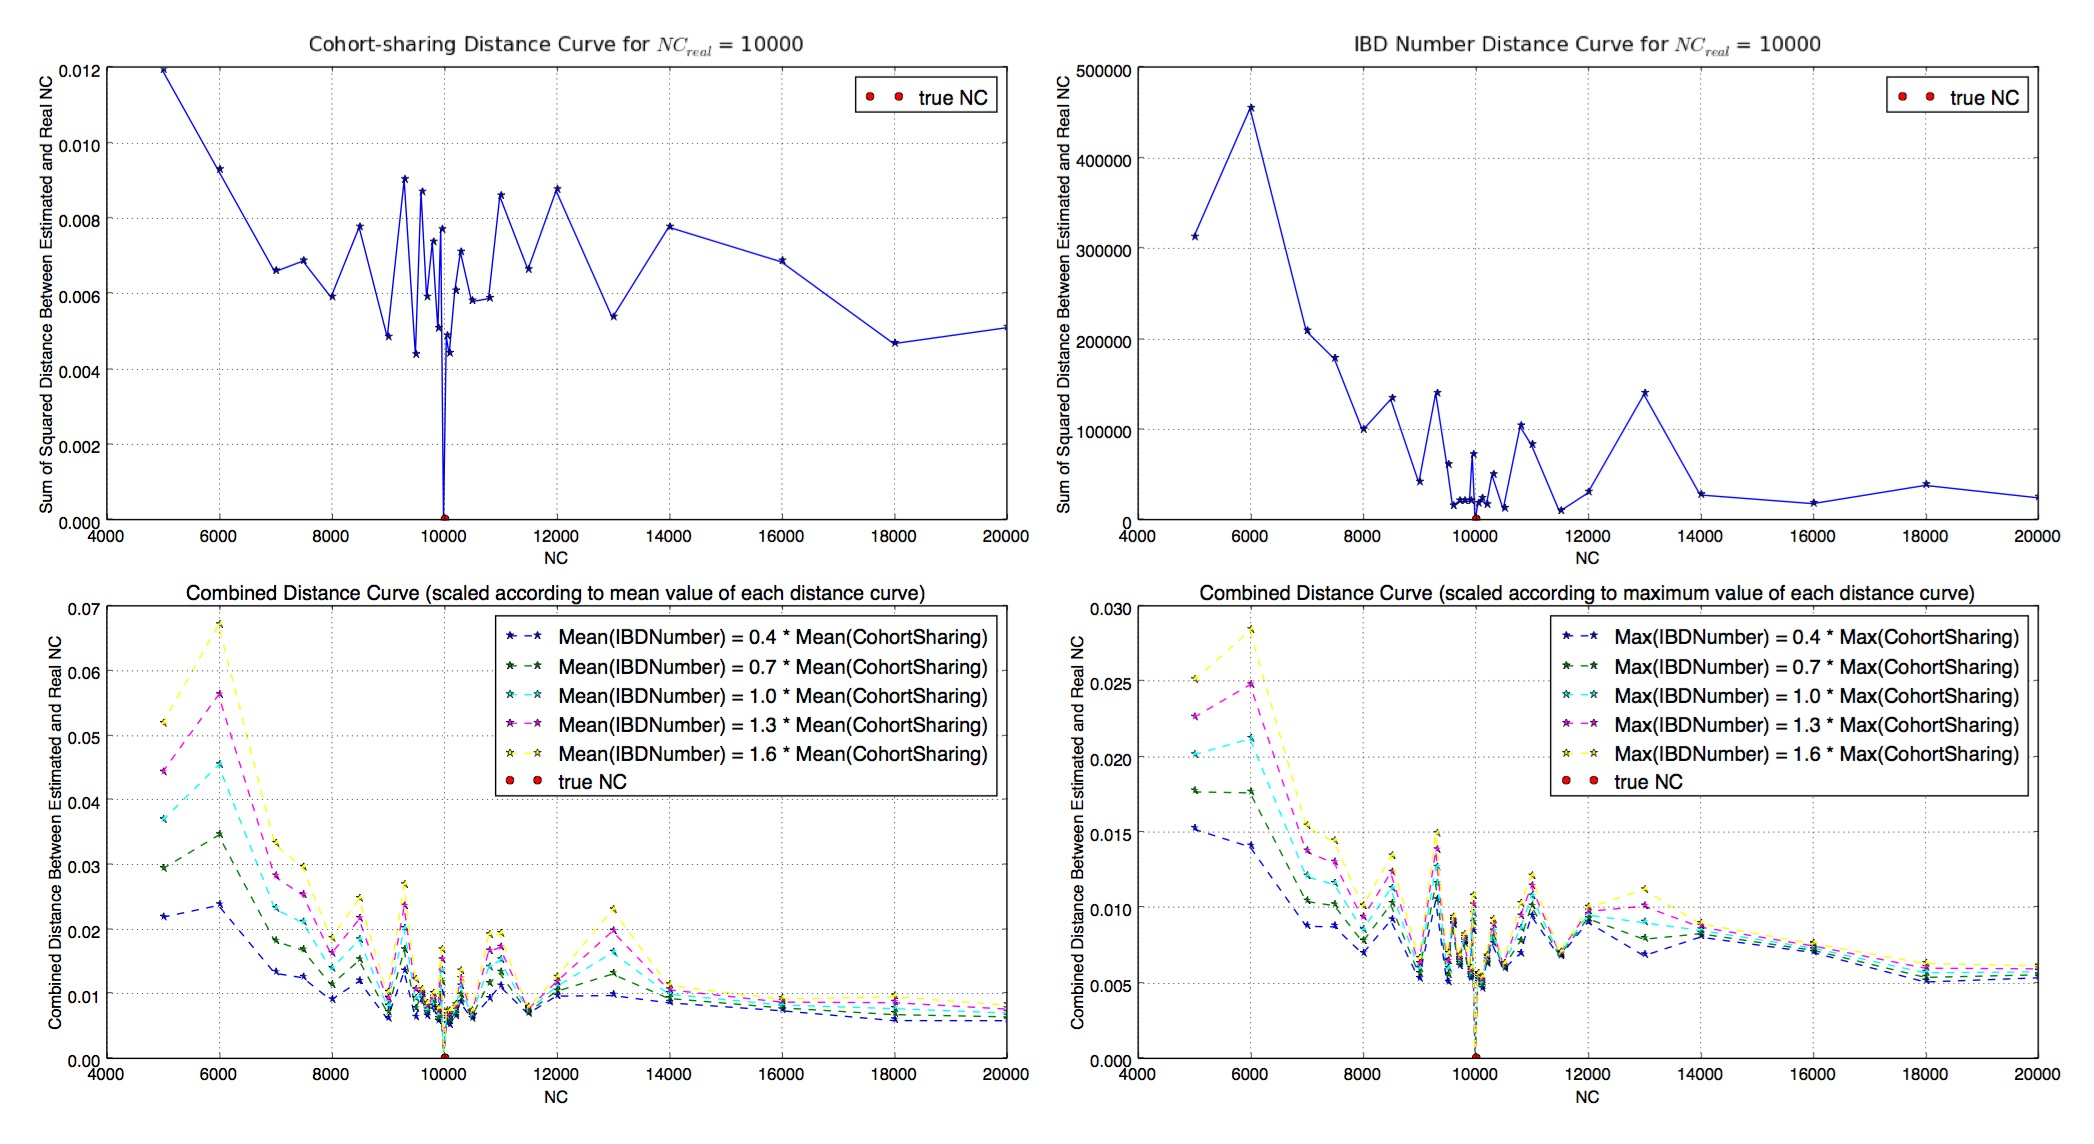
\includegraphics[width=280pt, height=170pt]{like_com_NC.jpg}}
\caption{Distance curves for $NC$. The above two curves are the distance curve for average IBD sharing and IBD segment number distribution, and the below two curves are the combined curve according to \textbf{Mean} and \textbf{Max} value, respectively.}\label{fig:dis_com_NC}
\end{figure}




\section{Discussion}

The new statistic actually doesn't flash out in the inference framework. Also, combining the new statistic with the old IBD number distribution won't help in the inference framework.

In the constant population size model, the average IBD sharing statistic is indeed a good indicator of the true population size. This is good. However, our old statistic (IBD segment number distribution) can also indicate the true population size. In that case, the new statistic doesn't do better than the old one.

In the bottleneck population size model, we are still not better than the old statistic with the new statistic. As we know, we have the following parameters to be evaluated in this bottleneck model:

\begin{enumerate}
\item $NA$: ancient population size;
\item $NC$: current population size;
\item $TB$: time to bottleneck event;
\item $NB$: bottleneck population size; or $T$: bottleneck duration;
\item $\frac{T}{NB}$: bottleneck strength
\end{enumerate}

In the following analysis and comparison, we will not show all the old results. But our comparison is objectively based on that. For $NA$ and $NC$, the old and the new statistics all can't determine their true value, as the distance curves are neither convex nor smooth. For $TB$, the new statistic is not able to indicate the true parameter, while the old statistic can do that. For $NB$ and $T$, if all other parameters are set to their true value, the old and the new statistics have the same performance, and for both the new and old statistics, these two parameters can always be retrieved even with imperfect information of $TB$. For the bottleneck strength, the results from the new statistic will be biased by the value of $TB$, while the results from the old statistic will not, and actually they can always be precisely estimated (See Figure~\ref{fig:TNBTB_old}). So, over all, the new statistic doesn't do better than the old one, though it shows same trend for some of those explored parameters.

\begin{figure}[h]
\centerline{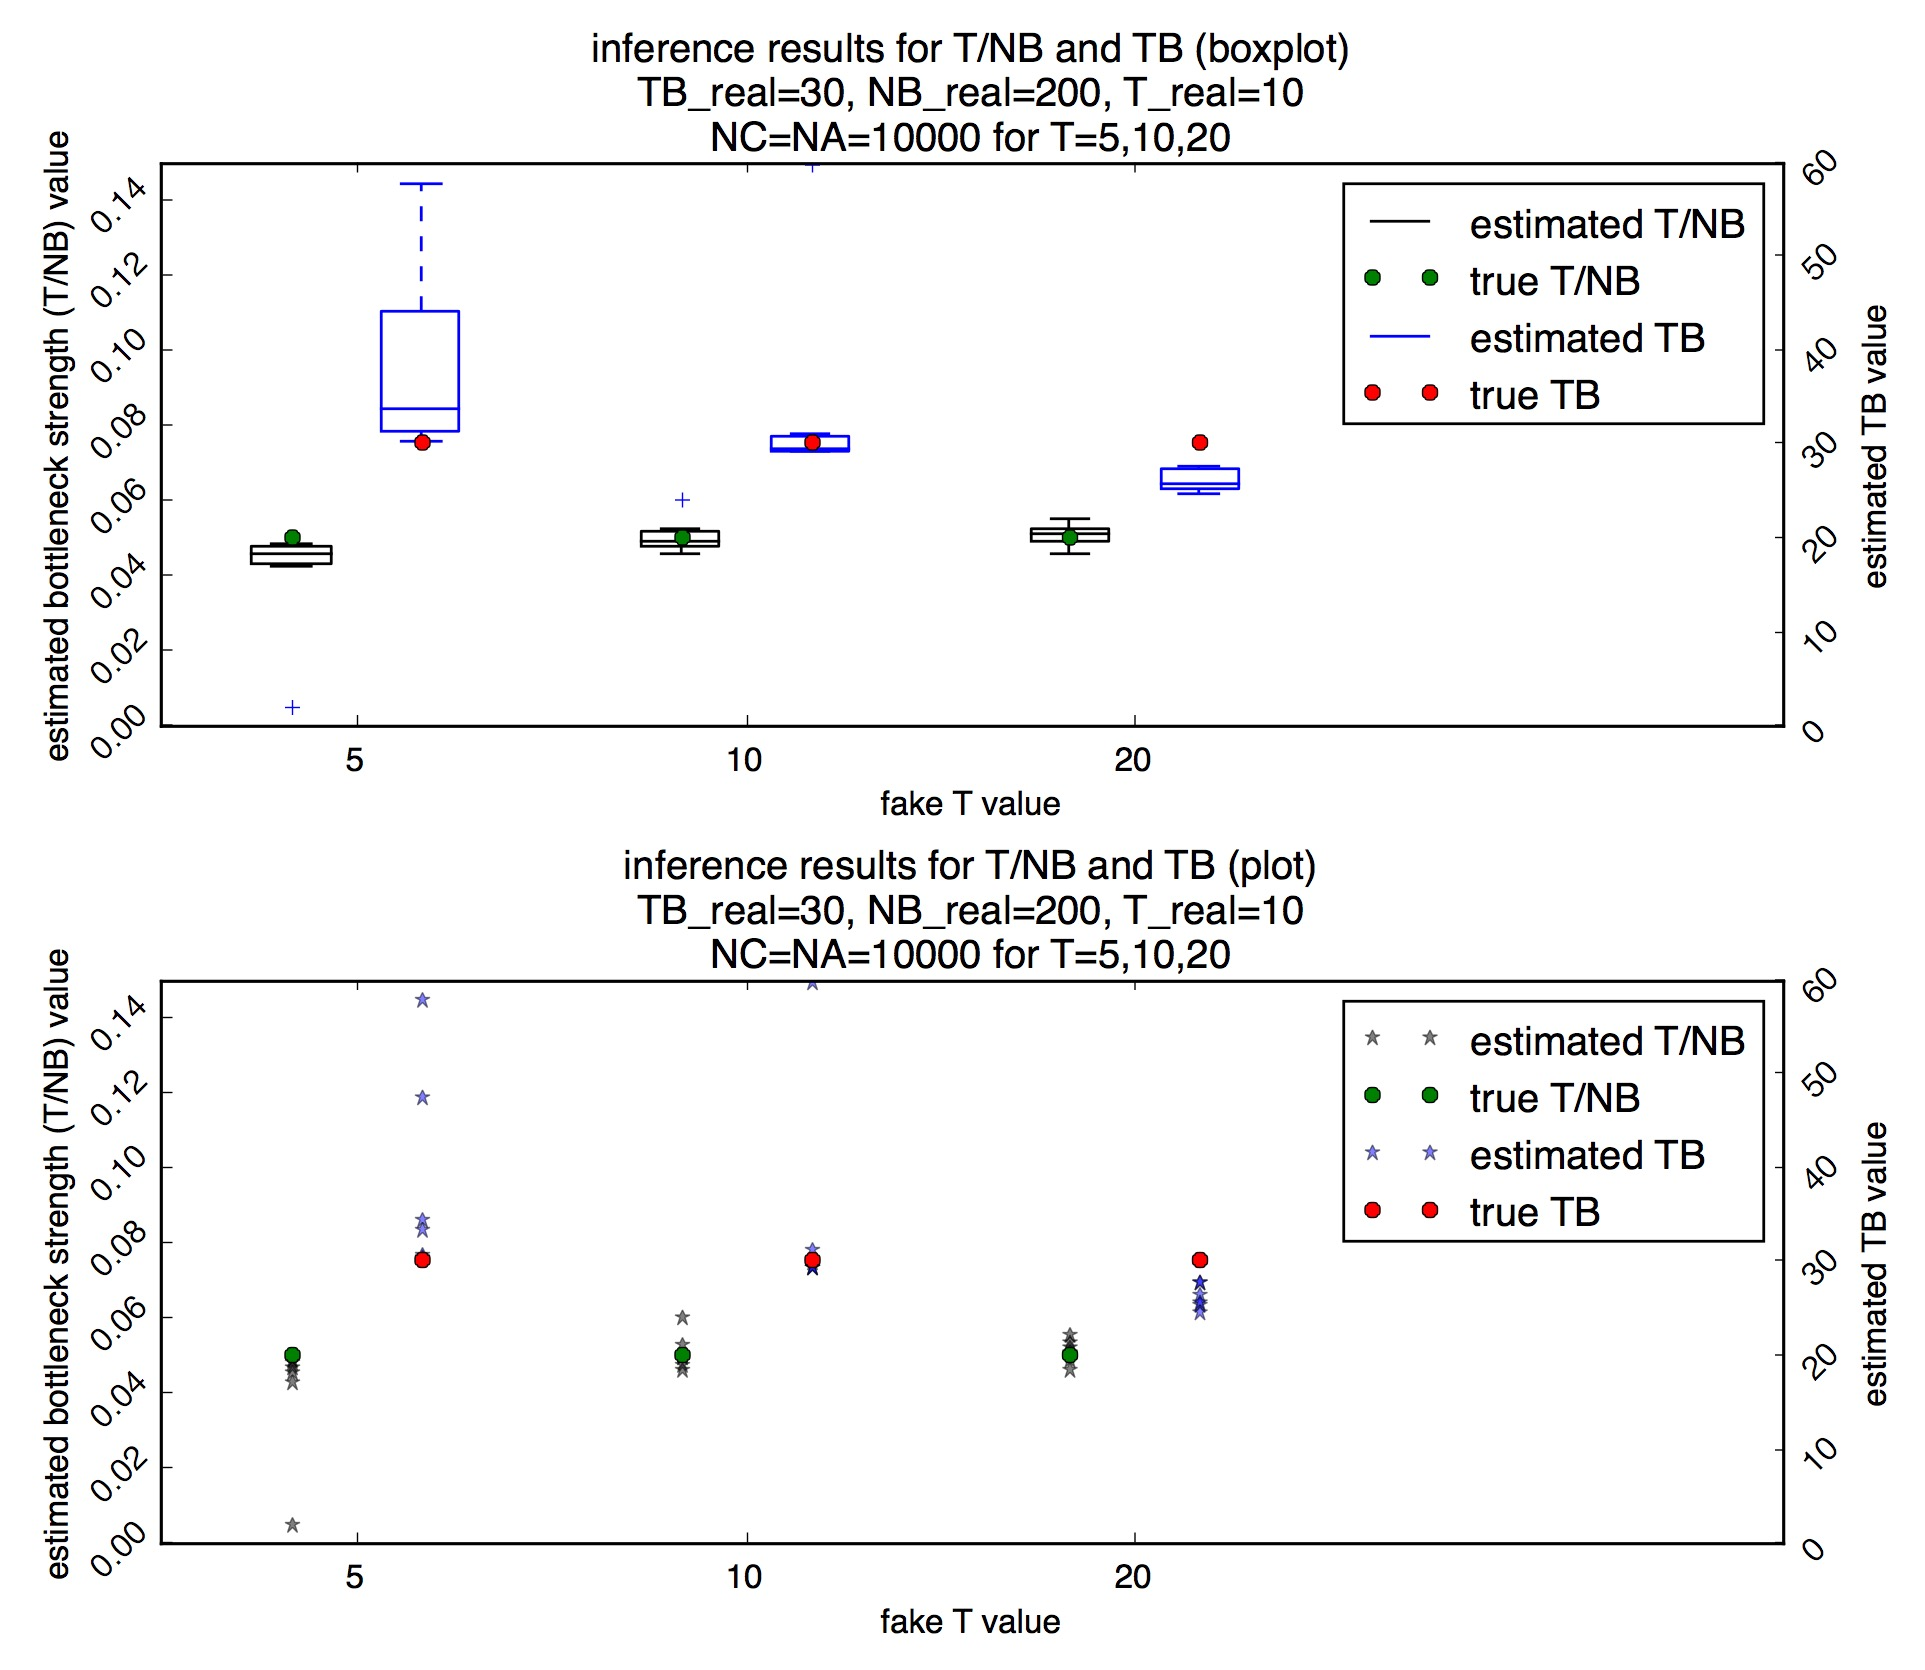
\includegraphics[width=250pt, height=210pt]{TNBTB_old.jpg}}
\caption{Estimation (old results) for $\frac{T}{NB}$ and $TB$ jointly, expressed in boxplot and plot format. We can see that, the estimation of $\frac{T}{NB}$ is always good, unbiased with $TB$. At the same time, the estimation of $TB$ jointly is feasible, though a little biased by the chosen value of $T$.}\label{fig:TNBTB_old}
\end{figure}

Also, from the results we see that, combining the two statistics won't help at all. So, overall, the new statistic doesn't help in such demographic inference.



\section{Conclusion}

In this project, we did extensive simulations to evaluate the average IBD sharing statistic used in demographic inference, via minimum-distance method. This new statistic doesn't perform better than the old one, as we discussed in the previous sections. And combining the new statistic with the old IBD segment number distribution won't give rise to a better precision for the inference. But as this project is on earth evaluation-oriented, it finishes our original target.

We hope in the future, we can have a more gentle start for a scientific project, with solid scientific intuition and motivation. Otherwise, it may not be that exciting, as most of the simple ideas are not correct in scientific research. Also, we will not reply on simulation-based approach too much, especially using it as our main research approach. Simulation is more appropriate for evaluating some theories, other than substituting them. At this point, out start is not as good as we expected.





\section*{Acknowledgement}
We thank Dr. Shai Carmi and the course team of COMS4761 (instructor Prof. Itsik Pe'er and TA Mr. Cameron Palmer) for useful discussions and suggestions for this project. We also thank the feedback from the classmates during the project presentation sections.

\paragraph{Funding\textcolon} This is a course project in Columbia University Computer Science, so no direct funding is issued.


\bibliographystyle{natbib}
%\bibliographystyle{achemnat}
%\bibliographystyle{plainnat}
%\bibliographystyle{abbrv}
%\bibliographystyle{bioinformatics}
%\bibliographystyle{plain}
\bibliography{document.bib}



\end{document}




% something else:
% table:
%\begin{table}[!t]
%\processtable{This is table caption\label{Tab:01}}
%{\begin{tabular}{llll}\toprule
%head1 & head2 & head3 & head4\\\midrule
%row1 & row1 & row1 & row1\\
%row2 & row2 & row2 & row2\\
%row3 & row3 & row3 & row3\\
%row4 & row4 & row4 & row4\\\botrule
%\end{tabular}}{This is a footnote}
%\end{table}

% equation:
%\begin{equation}
%\sum x+ y =Z\label{eq:01}
%\end{equation}